\documentclass{ieeeaccess}
\usepackage{cite}
\usepackage[utf8]{inputenc}
\usepackage[spanish]{babel}
\usepackage{amsmath,amssymb,amsfonts}
\usepackage{algorithmic}
\usepackage{graphicx}
\usepackage{textcomp}
\usepackage{multirow}
\usepackage{listings}

\def\BibTeX{{\rm B\kern-.05em{\sc i\kern-.025em b}\kern-.08em
    T\kern-.1667em\lower.7ex\hbox{E}\kern-.125emX}}
\begin{document}
\history{Date of publication xx 00, 0000, date of current version xxx 00, 0000.}
\doi{10.1109/ACCESS.2017.DOI}

\title{Péndulo Invertido}
\author{\uppercase{Andrea Posada Cárdenas\authorrefmark{1}},
  \uppercase{Santiago Hincapie Potes}\authorrefmark{2}}
\address[1]{Estudiante de Ingeniería Matemática, Universidad EAFIT,
  Medellin, Colombia (e-mail: aposad31@eafit.edu.co)}
\address[2]{Estudiante de Ingeniería Matemática, Universidad EAFIT,
  Medellin, Colombia (e-mail: shinca12@eafit.edu.co)}

\markboth{}
{Author \headeretal: Preparation of Papers for IEEE TRANSACTIONS and JOURNALS}
{Author \headeretal: Preparation of Papers for IEEE TRANSACTIONS and JOURNALS}

\corresp{Corresponding author: Andrea Posada Cárdenas
  (e-mail: aposad31@eafit.edu.co).}

\begin{abstract}
  TODO:Add abstract
\end{abstract}

\begin{keywords}
  TODO:Add keywords
\end{keywords}

\titlepgskip=-15pt

\maketitle

\section{Introducción}\label{sec:introduction}

El péndulo invertido sobre un carro representa un sistema que comúnmente es encontrado en los libros de control y en la literatura. Esto se debe en parte a que es inestable sin control, e.d., el péndulo caería si el carro no se moviese para balancearlo y a que es un sistema no lineal. El despegue de cohete está relacionado directamente con el sistema del péndulo invertido.\\

Se estudia el péndulo invertido en dos dimensiones, que se muestra en la Figura \ref{diagram}. La entrada de control es la fuerza $F$ que mueve el carro horizontalmente y las salidas son la posición angular del péndulo $\theta$ y la posición horizontal del carro $x$, siendo un sistema `single input, multiple output' SIMO. Las entradas, salidas y parámetros, su notación, significado físico y unidades de medida se presentan en el Cuadro \ref{tab: des}.

\begin{figure}[h!]
\centering
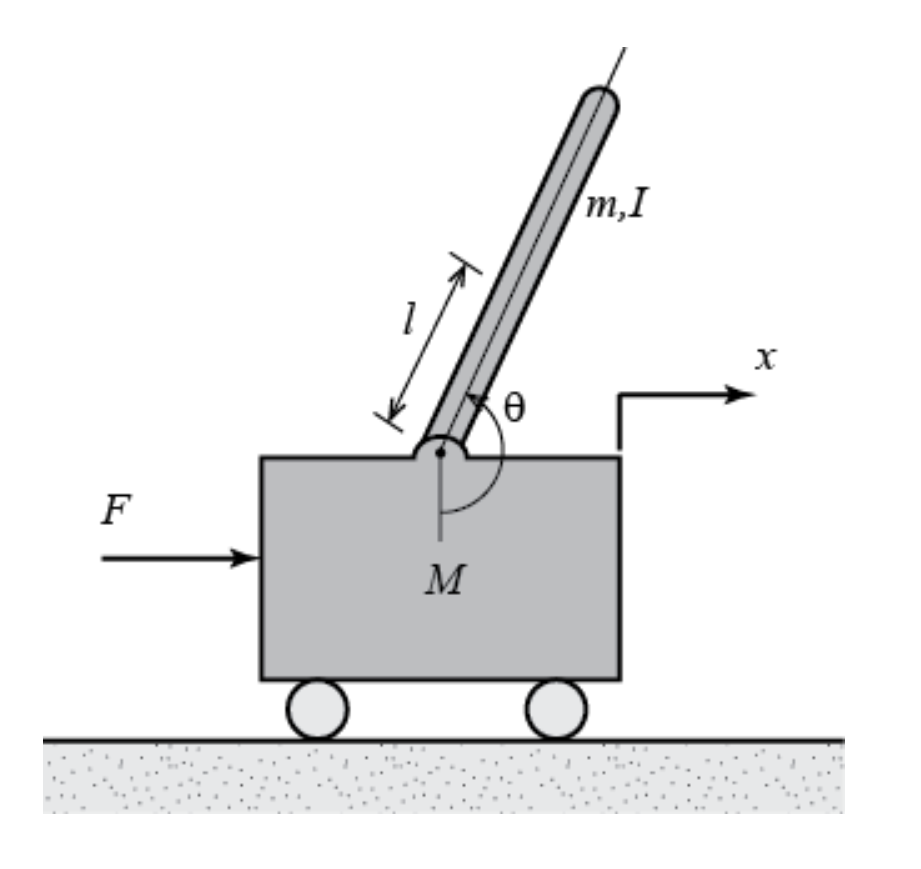
\includegraphics[scale=0.5]{pendulo.PNG}
%\caption{diagrama}
\label{diagram}
\end{figure}

\begin{table}[h!]
\centering
\caption{Parámetros, entradas y salidas}
\label{tab: des}
\begin{tabular}{|c|ll|c|}
\hline
\multicolumn{1}{|l|}{\textbf{}} & \multicolumn{1}{l|}{\textbf{Notación}} & \multicolumn{1}{c|}{\textbf{Significado}}  &     \multicolumn{1}{c|}{\textbf{Unidades}}    \\ \hline
\multirow{7}{*}{\rotatebox{90}{\textbf{Parámetros}}} & \multicolumn{1}{c|}{$M$}  & masa del carro      & kg        \\
                                    & \multicolumn{1}{c|}{$m$} & masa del péndulo     & kg        \\
                                    & \multicolumn{1}{c|}{$b$} & coeficiente de fricción       & N*m/s    \\
                                    & \multicolumn{1}{c|}{$I$} & momento de inercia del centro de masa     & kg         \\
                                    & \multicolumn{1}{c|}{} & del péndulo      &       \\
                                    & \multicolumn{1}{c|}{$L$} & longitud al centro de masa del péndulo  & m        \\
                                    & \multicolumn{1}{c|}{$g$} & gravedad      & m/$\textnormal{s}^2$        \\ \hline
\multirow{3}{*}{\rotatebox{90}{\textbf{Inputs}}} & \multicolumn{1}{c|}{} & &  \\
                                    & \multicolumn{1}{c|}{$F$}  & fuerza aplicada al carro & N         \\
                                    & \multicolumn{1}{c|}{} &  &      \\\hline
\multirow{4}{*}{\rotatebox{90}{\textbf{Outputs}}} & \multicolumn{1}{c|}{} & &  \\
                                    & \multicolumn{1}{c|}{$x$}  & posición del carro en el eje x & m         \\
                                    & \multicolumn{1}{c|}{$\theta$} & ángulo del péndulo desde la vertical (abajo) & rad        \\
                                   & \multicolumn{1}{c|}{} &  &         \\\hline                                
\end{tabular}
\end{table}

\subsection{Análisis diagrama de cuerpo libre y sistema de ecuaciones}

El diagrama de cuerpo libre se presenta en la Figura \ref{cuerpo}.\\

\begin{figure}[h!]
\centering
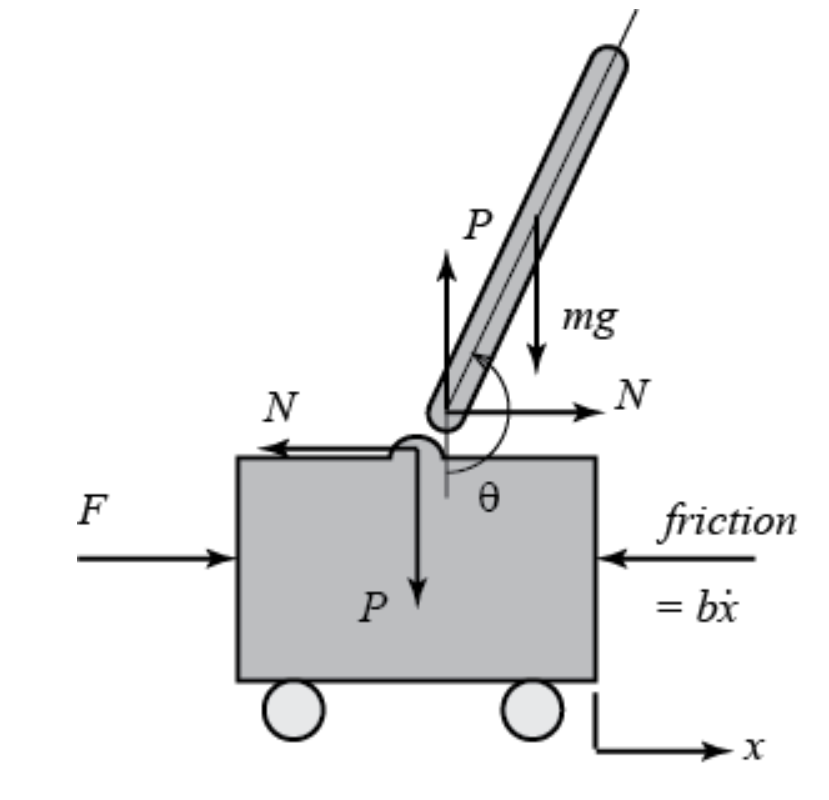
\includegraphics[scale=0.5]{diagrama_cuerpo.PNG}
\label{cuerpo}
\end{figure}

Sumando las fuerzas horizontales se obtiene la siguiente ecuación de movimiento

\begin{equation}
\label{eq: motion}
M\ddot{x}+b\dot{x}+N = F
\end{equation}
donde $$N=m\ddot{x}+ml\ddot{\theta}\cos(\theta)-ml\dot(\theta)^2\sin(\theta)$$ que se obtiene de la suma de las fuerzas horizontales en el diagrama de cuerpo libre del péndulo.\\

Sustituyendo $N$ en la ecuación (1), se obtiene
\begin{equation}
\label{eq: motion1}
(M+m)\ddot{x}+b\dot{x}+ml\ddot{\theta}\cos(\theta)-ml\dot{\theta}^2\sin(\theta) = F
\end{equation}

Por otro lado, sumando las fuerzas verticales en el diagrama diagrama de cuerpo libre del péndulo y los momentos alrededor del centroide del péndulo, se tiene, respectivamente
$$P\sin(\theta)+N\cos(\theta)-mg\sin(\theta)=ml\ddot{\theta}+m\ddot{x}\cos(\theta)$$
$$Pl\sin(\theta)-Nl\cos(\theta)=I\ddot{\theta}$$

Remplazando la ecuación de la suma de los momentos en la de la suma de las fuerzas verticales (ecuaciones anteriores), se obtiene 
\begin{equation}
\label{eq: motion2}
(I+ml^2)\ddot{\theta}+mgl\sin(\theta)=-ml\ddot{x}\cos(\theta)
\end{equation}

Las ecuaciones (\ref{eq: motion1}) y (\ref{eq: motion2}) son las ecuaciones que describen el sistema. 

\section{Sistema no lineal}
\subsection{Variables}
\label{subsub: var}
\begin{flalign*}
%\centering
\raggedright
  x_1 &= x       & \text{posición del carro}    \\
  x_2 &= \dot{x} & \text{velocidad del carro}    \\
  x_3 &= \theta       & \text{ángulo del péndulo desde la vertical}   \\
  x_4 &= \dot{\theta} & \text{velocidad angular del péndulo} \\
  u   &= F       & \text{Fuerza de entrada}
\end{flalign*}

\subsection{Espacio de estados no lineal}
Partiendo de las ecuaciones de movimiento (\ref{eq: motion1}) y (\ref{eq: motion2}), se redefine el sistema de ecuaciones de la siguiente manera, teniendo en cuenta la notación introducida anteriormente en \ref{subsub: var}.

\begin{eqnarray}
\label{eq: sistema}
\left\{
\begin{array}{ll}
	f_1=\displaystyle\dot{x_1} = \displaystyle x_2\\
    f_2=\displaystyle\dot{x_2} = \displaystyle\frac{(I+ml^2)a+m^2l^2g\sin(x_3)\cos(x_3)}{(M+m)(I+ml^2)-m^2l^2\cos^2(x_3)}\\ 
    f_3=\displaystyle\dot{x_3} = \displaystyle x_4\\
    f_4=\dot{x_4} = \displaystyle\frac{-ml\cos(x_3)a-(M+m)mlg\sin(x_3)}{(M+m)(I+ml^2)-m^2l^2\cos^2(x_3)}\\
\end{array}
\right.
\end{eqnarray}
donde $a = u-bx_2+mlx_4^2\sin(x_3)$\\

$\dot{x_2}$ y $\dot{x_4}$ se obtienen despejando $\ddot{x}$ y $\ddot{\theta}$ de las ecuaciones (\ref{eq: motion1}) y (\ref{eq: motion2}), como se muestra a continuación, y teniendo en cuenta que $\ddot{x}=\dot{x_2}$ y $\ddot{\theta}=\dot{x_4}$

\begin{eqnarray}
\label{eq: x_2}
\dot{x_2} = \displaystyle\frac{u-bx_2-ml\dot{x_4}\cos(x_3)+mlx_4^2\sin(x_3)}{M+m}\\
\label{eq: x_4}
\dot{x_4} = \displaystyle\frac{-ml\dot{x_2}\cos(x_3)-mlg\sin(x_3)}{I+ml^2}
\end{eqnarray}\\

Al reemplazar el valor de $\dot{x_4}$, ecuación (\ref{eq: x_4}), en la ecuación (\ref{eq: x_2}), haciendo álgebra y juntando términos semejantes se obtiene la expresión del sistema de ecuaciones (\ref{eq: sistema}) para $\dot{x_2}$. Repitiendo el mismo proceso pero para el valor de $\dot{x_2}$, ecuación (\ref{eq: x_2}), en la ecuación (\ref{eq: x_4}) se obtiene la expresión señalada en el sistema de ecuaciones (\ref{eq: sistema}) para $\dot{x_4}$

\subsection{Salidas}
El sistema de ecuaciones (\ref{eq: salidas}) es la representación de las salidas del sistema.
\begin{eqnarray}
\label{eq: salidas}
\left\{
\begin{array}{ll}
	h_1=x_1\\
    h_2=x_3\\
\end{array}
\right.
\end{eqnarray}

\subsection{Diagrama de bloques de \textit{Simulink - MATLAB}}

El péndulo invertido sobre un carro se implementó en \textit{Simulink} de \textit{MATLAB}. Se presentan el diagrama de bloques, \ref{diagramabloques}, la expansión del subsistema, \ref{subsistema}, y el código de \textit{MATLAB} de la fcn, que es simplemente la implementación del sistema de ecuaciones (\ref{eq: sistema}). Los párametros no aparecen con los valores empleados, dado que la asignación de estos, al igual que la de las condiciones iniciales se realiza mediante una máscara.

\begin{figure}[h!]
\centering
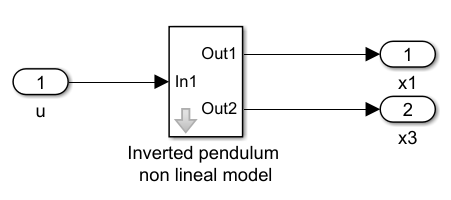
\includegraphics[scale=1]{diagrama_bloques.PNG}
\label{diagramabloques}
\end{figure}

\begin{figure}[h!]
\centering
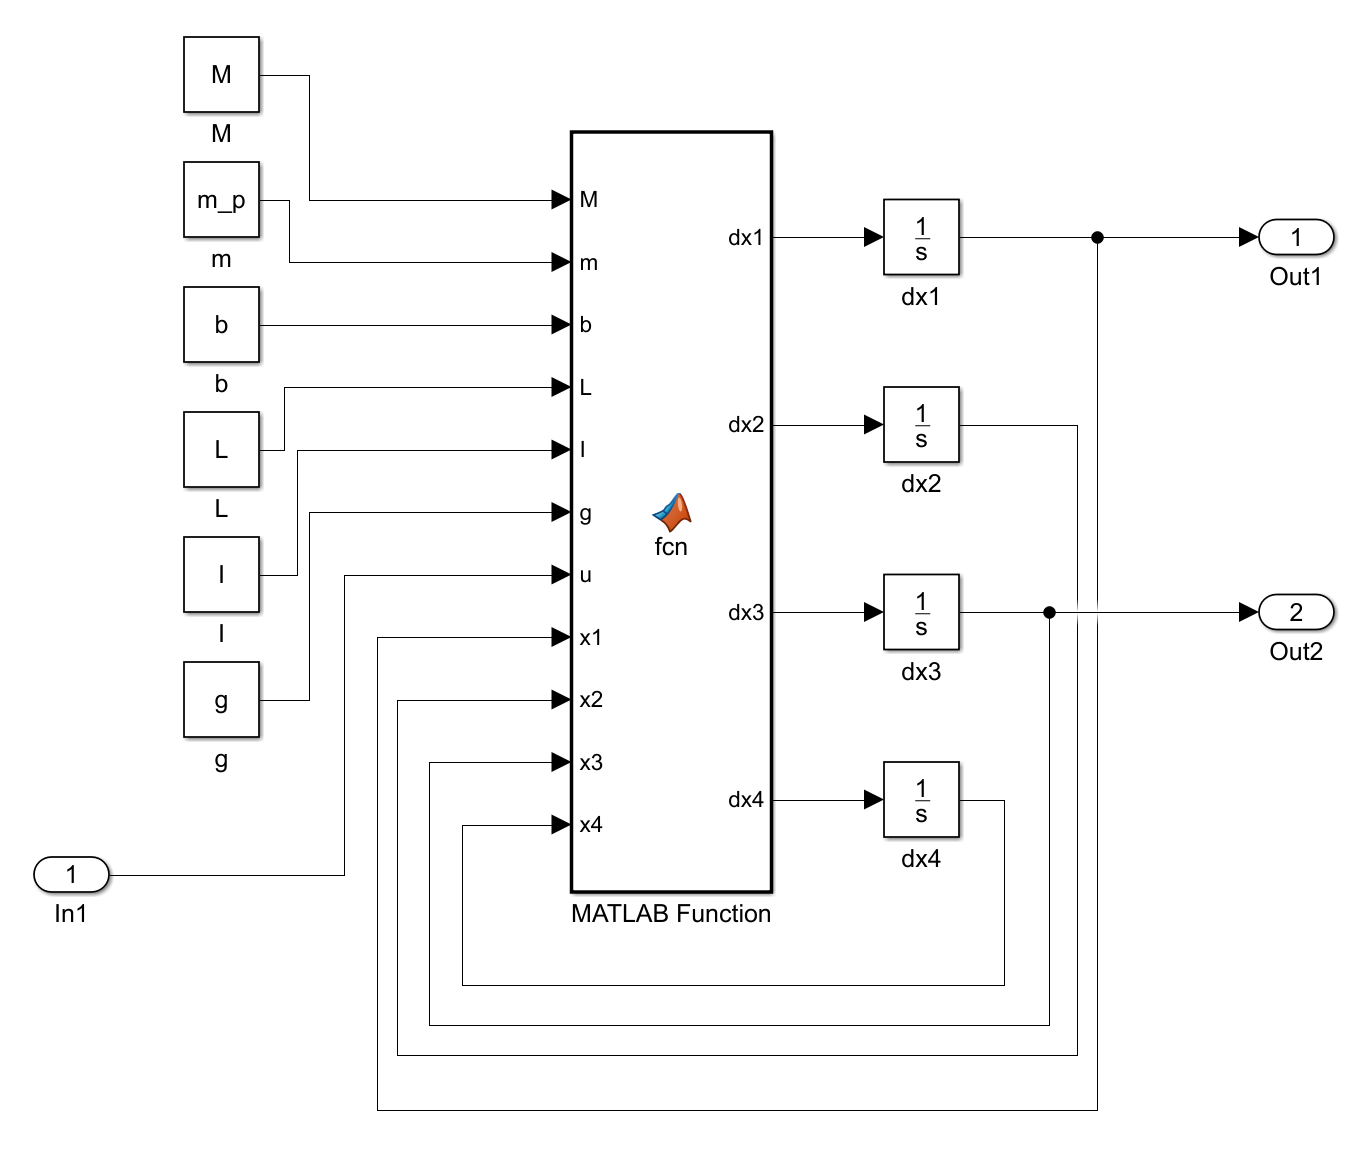
\includegraphics[scale=0.6]{diagrama_bloques_subsistema.PNG}
\label{subsistema}
\end{figure}


\lstset{language=Matlab, breaklines=true, basicstyle=\footnotesize}
\lstset{numbers=left, numberstyle=\tiny, stepnumber=1, numbersep=-2pt}
\begin{lstlisting}[frame=single]
function [dx1, dx2, dx3, dx4] = fcn(M, m, b, L, I, g, u, x1, x2, x3, x4)
    denominator = (M+m)*(I+m*L^2)-m^2*L^2*cos(x3)^2;
    dx1 = x2;
    dx2 = ((I+m*L^2)*(u-b*x2+m*L*x4^2*sin(x3))+m^2*L^2*g*sin(x3)*cos(x3))/denominator;
    dx3 = x4;
    dx4 = (-m*L*u*cos(x3)+m*L*b*x2*cos(x3)-m^2*L^2*x4^2*sin(x3)*cos(x3)-(M+m)*m*g*L*sin(x3))/denominator;
end
\end{lstlisting}
\section{Simulación}
\subsection{Solución numérica}
%\begin{figure}
%\label{fig:numet}
%\includegraphics[scale=0.5]{num-met.pgf}
%\end{figure}
\subsubsection{Método de Euler}
en la figura~\ref{fig:numet} se puede ver la comparación del resultado
obtenido al realizar la simulación con el método de Euler, con un
paso $h = \frac{1}{4000}$, esto debido a que con valores mas altos
la diferencia entre ambas simulaciones se vuelve bastante notoria.
Estas diferencias pueden deberse a la alta complejidad de las
ecuaciones de estado, por lo cual se vuelve necesario utilizar un
paso bastante pequeño.
\subsubsection{Método de Runge-Kutta}
Para el método de Runge-Kutta de cuarto orden, el paso utilizado es
de $h = \frac{1}{10}$, la precisión obtenida es tal que en la figura
no se logra observar fácilmente la simulación arrojada por simulink,
esto indica que el método de Runge-Kutta posee un orden de error
bastante bajo, por lo cual se puede decir que realiza buenas
aproximaciones de las ecuaciones de estados.
Es importante resaltar que al utilizar un paso relativamente grande,
el tiempo de computo asociado al método es bastante bajo.

\subsection{Cambio de parámetros}
Para analizar la sensibilidad del modelo a ciertos parámetros, se
consideró el efecto del cambio sobre dos parámetros del modelo,
la longitud al centro de masa del péndulo y la masa del péndulo,
esto debido a que experimentalmente hablando es bastante sencillo y
económico remplazar esta componentes del péndulo.
\subsubsection{Longitud al centro de masa}
%\begin{figure}
%  \label{fig:var-len}
%  \includegraphics{len.pgf}
%\end{figure}
En la figura~\ref{fig:var-len} se varía la distancia del centro de masa
del péndulo. De esta se puede observar que la amplitud con la que se
mueve el carro disminuye a medida que disminuye la distancia del centro
de masa del péndulo, esto se debe a que la inercia depende de esta
distancia y es esta la que provoca dichos movimientos sobre el carro.
Por otro lado. Por otro lado, es posible notar que el angulo del péndulo
no se ve muy afectado por esta longitud.
\section{Linealización}

\subsection{Puntos de equilibrio}
Igualando las $f_n$ a 0, para $n=1,2,3,4$, se obtienen seis puntos de equilibrio, mostrados en el Cuadro \ref{tab: ptoseq}.

\begin{table}[h!]
\centering
\caption{Puntos de equilibrio}
\label{tab: ptoseq}
\begin{tabular}{|c|c|c|}
\hline
\textbf{} & \textbf{Variable} & \textbf{Valor}\\\hline
\multirow{5}{*}{\textbf{1}} & $x_1$ & 0\\
							& $x_2$ & 0\\
                            & $x_3$ & $- \pi + 2\arctan((33^{1/2}\cdot n)/11 - (154^{1/2}*\cdot n)/11)$\\
                            & $x_4$ & 0\\
                            & $x_5$ & $(154^{1/2}\cdot 49i)/100$\\\hline

\multirow{5}{*}{\textbf{2}} & $x_1$ & 0\\
							& $x_2$ & 0\\
                            & $x_3$ & $-2\cdot\arctan((33^{1/2}\cdot n)/11 - (154^{1/2}\cdot n)/11)$\\
                            & $x_4$ & 0\\
                            & $x_5$ & $-(154^{1/2}\cdot 49i)/100$\\\hline

\multirow{5}{*}{\textbf{3}} & $x_1$ & 0\\
							& $x_2$ & 0\\
                            & $x_3$ & $2\cdot\arctan((33^{1/2}\cdot n)/11 - (154^{1/2}\cdot n)/11)$\\
                            & $x_4$ & 0\\
                            & $x_5$ & $(154^{1/2}\cdot 49i)/100$\\\hline

\multirow{5}{*}{\textbf{4}} & $x_1$ & 0\\
							& $x_2$ & 0\\
                            & $x_3$ & $\pi$\\
                            & $x_4$ & 0\\
                            & $x_5$ & 0\\\hline
                            
\multirow{5}{*}{\textbf{4}} & $x_1$ & 0\\
							& $x_2$ & 0\\
                            & $x_3$ & 0\\
                            & $x_4$ & 0\\
                            & $x_5$ & 0\\\hline
                            
\multirow{5}{*}{\textbf{4}} & $x_1$ & 0\\
							& $x_2$ & 0\\
                            & $x_3$ & $\pi - 2\cdot\arctan((33^{1/2}\cdot n)/11 - (154^{1/2}\cdot i)/11)$\\
                            & $x_4$ & 0\\
                            & $x_5$ & $-(154^{1/2}\cdot 49i)/100$\\\hline
\end{tabular}
\end{table}

\subsection{Sistema linealizado}
Un sistema lineal es de la forma
$$\dot{X}=AX+BU$$
$$Y=CX+DU$$
donde $Y$ es el vector de salidas, $X$ es el vector de estados, $U$ es el vector de entradas y $A$, $B$, $C$ y $D$ son matrices (o vectores dependiendo de las dimensiones de $X$ y $U$) de coeficientes constantes.\\

Tanto la linealización analítica como la linealización realizada con \textit{MATLAB} utilizando el modelo de bloques de \textit{Simulink}, se hacen con respecto al punto de equilibrio $x_1=0$, $x_2=0$, $x_3=0$, $x_4=0$ y $u=0$.

\subsubsection{Linealización analítica}

Se obtiene el sistema
\begin{eqnarray}
\Delta\dot{X} = A\Delta X + B\Delta U\\
\Delta Y = C\Delta X + D\Delta U
\end{eqnarray}
donde
$$A = \begin{bmatrix}
    0 & 1 & 0 & 0\\
    0 & -2/11 & 147/55 & 0\\
    0 & 0 & 0 & 1\\
    0 & 5/11 & -343/11 & 0
\end{bmatrix}$$
$$B = \begin{bmatrix}
    0 &
    20/11 &
    0 &
    -50/11
\end{bmatrix}^{T}$$
$$C = \begin{bmatrix}
    1 & 0 & 0 & 0\\
    0 & 0 & 1 & 0
\end{bmatrix}$$
$$D = \begin{bmatrix}
    0&
    0
\end{bmatrix}^{T}$$
\subsubsection{Linealización con \textit{Simulink}}
% Aqui tengo algo que poner, escribe y me dejas un espacio.
\subsection{Curva de linealidad}
\EOD{}
\end{document}